\documentclass{beamer}
\usepackage[utf8]{inputenc}
\usepackage[T1]{fontenc}
\usepackage[slovene]{babel}
\usepackage{lmodern}
\usepackage{url}
\usepackage{graphicx}

% 1. naloga: pripravite naslovno stran
% Nekaj o kompleksni dinamiki
% Beno Učakar
% Fakulteta za matematiko in fiziko
\title{Nekaj o kompleksni dinamiki}
\author{Beno Učakar}

\date{14.2.2024}



\usetheme{metropolis}
\usecolortheme{spruce}
\usefonttheme{structurebold}
\useoutertheme{infolines}
\beamertemplatenavigationsymbolsempty

% 2. naloga: definirajte novo AMS okolje "definicija"
{\theoremstyle{definition}
\newtheorem{definicija}{Definicija}
}


\begin{document}


\maketitle% 1. naloga: pripravite naslovno stran

\begin{frame}
    Kompleksna števila lahko enostavno vstavimo v polinom, kaj pa druge funkcije? 
    Za primer si poglejmo, kako izračunamo $e^{i\theta}$ s pomočjo Taylorjeve vrste.
    
    % 3. naloga: okolje za poravnano enačbo
   
        
        \begin{align*}
             e^{i\theta} & = \sum_{n=0}^{\infty} \frac{(i\theta)^n}{n!} \\
                         & = 1 + i\theta - \frac{\theta^2}{2!} - \frac{i\theta^3}{3!} + \frac{\theta^4}{4!} + \frac{i\theta^5}{5!} + \ldots \\
                         & = \left( 1 - \frac{\theta^2}{2!} + \frac{\theta^4}{4!} - \ldots \right) 
                            + i \left(\theta - \frac{\theta^3}{3!} + \frac{\theta^5}{5!} - \ldots \right) \\
                         & = \cos(\theta) + i\sin(\theta).
        \end{align*}
 
\end{frame}

\begin{frame}

    % 2. naloga: uporabite okolje definicija in poudarite izraz "večkratnost"
    % začetek definicije
        
        \begin{definicija}
            Naj bo $f \in O(D)$ in $z_0 \in D$ fiksna točka funkcije $f$.
            Število $\lambda = f'(z_0)$ imenujemo \textbf{večkratnost} funkcije $f$ v točki $z_0$.
        \end{definicija}
    % konec definicije
    
    % 4. naloga: prelom prosojnice

    \begin{exampleblock}<2->{Glede na $\lambda$ karakteriziramo fiksne točke:}
        % 4. naloga: postopno prikazovanje elementov in manjkajoč izraz
        \begin{enumerate} 
            \item<2-> $|\lambda| = 0$ je \textbf{super privlačna} fiksna točka.
            \item<3-> $|\lambda| < 1$ je \textbf{privlačna} fiksna točka.
            \item<4-> $|\lambda| > 1$ je \textbf{odbojna} fiksna točka.
            \item<5-> $|\lambda| = 1$: 
                če je $\lambda^n \neq 1$ za vsak $n \in \mathbf{N}$ je fiksna točka \textbf{iracionalno},
                sicer pa \textbf{racionalno nevtralna}.
        \end{enumerate}
    \end{exampleblock}
\end{frame}

\begin{frame}{Primer Julijeve množice}
    % 5. naloga: naslov prosojnice
    % Primer Julijeve množice
\begin{figure}
    \centering
    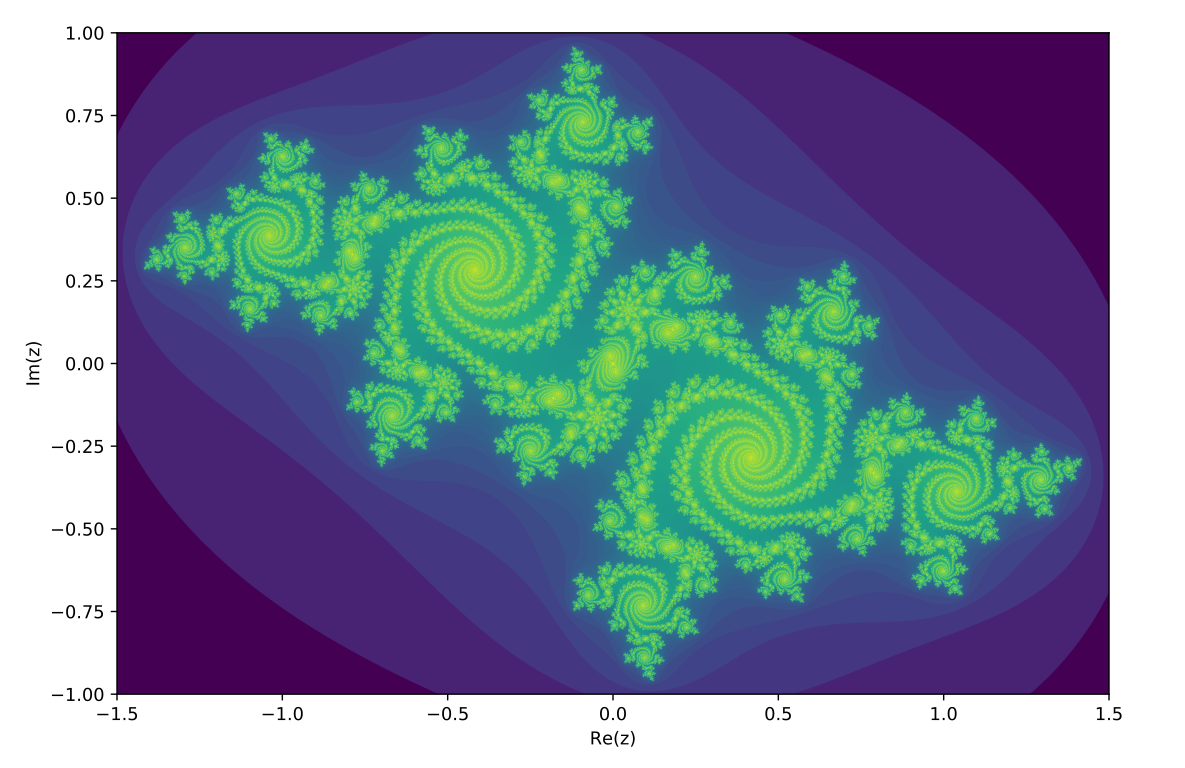
\includegraphics[scale=0.25]{julia_set.png}
\end{figure}
    % 5. naloga: vstavite sliko julia_set.png
\end{frame}

\end{document}